\documentclass[11pt]{article}

\usepackage[a4paper,margin=0.85in,headheight=15pt]{geometry}
\usepackage{fontspec}
\setmainfont{Latin Modern Roman}
\setsansfont{Latin Modern Sans}
\setmonofont{Latin Modern Mono}

\usepackage[table]{xcolor}
\usepackage{booktabs}
\usepackage{longtable}
\usepackage{tabularx}
\usepackage{array}
\usepackage{enumitem}
\usepackage{graphicx}
\usepackage{caption}
\usepackage{subcaption}
\usepackage{tikz}
\usetikzlibrary{arrows.meta,positioning,calc,fit,shapes.geometric,backgrounds,matrix}
\usepackage{pgfplots}
\usepackage{pgfplotstable}
\pgfplotsset{compat=1.18}
\usepackage{siunitx}
\sisetup{detect-all,group-separator={,},group-minimum-digits=4}
\usepackage{listings}
\usepackage{fancyhdr}
\usepackage{xurl}
\usepackage{hyperref}
\usepackage[backend=biber,style=numeric,sorting=none]{biblatex}
\addbibresource{../shared/sources.bib}

\definecolor{UMLBlue}{HTML}{1F5A7A}
\definecolor{UMLTeal}{HTML}{287D7D}
\definecolor{UMLGreen}{HTML}{2E7D32}
\definecolor{UMLAmber}{HTML}{B36B00}
\definecolor{UMLRed}{HTML}{A83232}
\definecolor{UMLInk}{HTML}{182026}
\definecolor{UMLMuted}{HTML}{66717A}
\definecolor{UMLPanel}{HTML}{F3F6F8}
\definecolor{UMLGrid}{HTML}{D9E1E7}

\newcommand{\ProjectTitle}{User Mode Linux Redesign}
\newcommand{\ProjectSubtitle}{Architecture, Implementation State, and Validation Evidence}
\newcommand{\ArtifactStatus}{Historical reporting artifact}
\newcommand{\CurrentTruthNotice}{This artifact is archived at its May 2026 reporting cutoff. Current UML v2 status lives in \texttt{Documentation/virt/uml/redesign/STATUS.md} and the live sequencing inventory, not in this report or deck.}
\newcommand{\ReportDate}{May 19, 2026}
\newcommand{\CutoffCommit}{9ccbf5e7bb58}
\newcommand{\BranchName}{umlctl-deploy}
\newcommand{\KVM}{\textsf{KVM}}
\newcommand{\UML}{\textsf{UML}}
\newcommand{\Seccomp}{\texttt{seccomp}}
\newcommand{\KVMvTwo}{\texttt{kvm-v2}}
\newcommand{\umlpath}[1]{\texttt{#1}}
\newcommand{\statusdone}{\textcolor{UMLGreen}{DONE}}
\newcommand{\statusprogress}{\textcolor{UMLAmber}{IN PROGRESS}}
\newcommand{\statusblocked}{\textcolor{UMLRed}{BLOCKED}}
\newcommand{\ratio}[1]{\ensuremath{#1\times}}


\hypersetup{
  colorlinks=true,
  linkcolor=UMLBlue,
  citecolor=UMLTeal,
  urlcolor=UMLBlue,
  pdftitle={\ProjectTitle: \ProjectSubtitle},
  pdfauthor={M. J. Bommarito}
}

\pagestyle{fancy}
\fancyhf{}
\lhead{\ProjectTitle}
\rhead{\ReportDate}
\cfoot{\thepage}

\setlist[itemize]{leftmargin=1.35em}
\setlist[enumerate]{leftmargin=1.45em}
\renewcommand{\arraystretch}{1.18}
\newcolumntype{Y}{>{\raggedright\arraybackslash}X}
\newcolumntype{L}[1]{>{\raggedright\arraybackslash}p{#1}}

\newcommand{\statuspill}[2]{%
  \begingroup
  \setlength{\fboxsep}{3pt}%
  \colorbox{#1!12}{\textcolor{#1}{\footnotesize\textbf{#2}}}%
  \endgroup
}
\newcommand{\donepill}{\statuspill{UMLGreen}{DONE}}
\newcommand{\progresspill}{\statuspill{UMLAmber}{IN PROGRESS}}
\newcommand{\blockedpill}{\statuspill{UMLRed}{BLOCKED}}
\newcommand{\plannedpill}{\statuspill{UMLBlue}{PLANNED}}
\newcommand{\metriccard}[3]{%
  \begin{minipage}[t]{0.235\linewidth}
  \centering
  \colorbox{#1!12}{\begin{minipage}{0.92\linewidth}
    \centering\vspace{0.45em}
    {\Large\textbf{\textcolor{#1}{#2}}}\\[0.25em]
    {\footnotesize #3}
    \vspace{0.45em}
  \end{minipage}}
  \end{minipage}
}

\title{\textbf{\ProjectTitle}\\[0.35em]\large \ProjectSubtitle}
\author{Reporting cutoff: branch \texttt{\BranchName}, commit \texttt{\CutoffCommit}}
\date{\ReportDate}

\begin{document}
\maketitle
\begin{center}
\fbox{\begin{minipage}{0.92\linewidth}
\textbf{\ArtifactStatus.} \CurrentTruthNotice
\end{minipage}}
\end{center}

\begin{abstract}
This report summarizes the User Mode Linux redesign branch as of
\ReportDate. It is a state report for maintainers: the first pages
state the branch claim, the delta from inherited \UML{}, and the
current validation position; later sections provide design detail,
benchmark data, validation evidence, and remaining work. The central
claim is that the redesign has moved beyond paper architecture:
backend abstraction, static-key gates, profile work, the Rust launcher,
and a substantial \KVMvTwo{} backend are present in-tree. The remaining
formal gate is sustained validation and upstream packaging.
\end{abstract}

\newpage
\section{Executive Summary}

\subsection{Goal and Current Position}

This branch proposes a profile-driven direction for \UML{} while
preserving the existing contract: the upstream Linux kernel built as
\texttt{arch/um} and executed as a host process. The target is not
another virtual machine monitor, not a container runtime, and not a
Linux reimplementation. The branch-local work is the combination of
swappable execution backends, runtime instrumentation gates,
profile-driven builds, and validation artifacts from one source tree.

\begin{figure}[h]
\centering
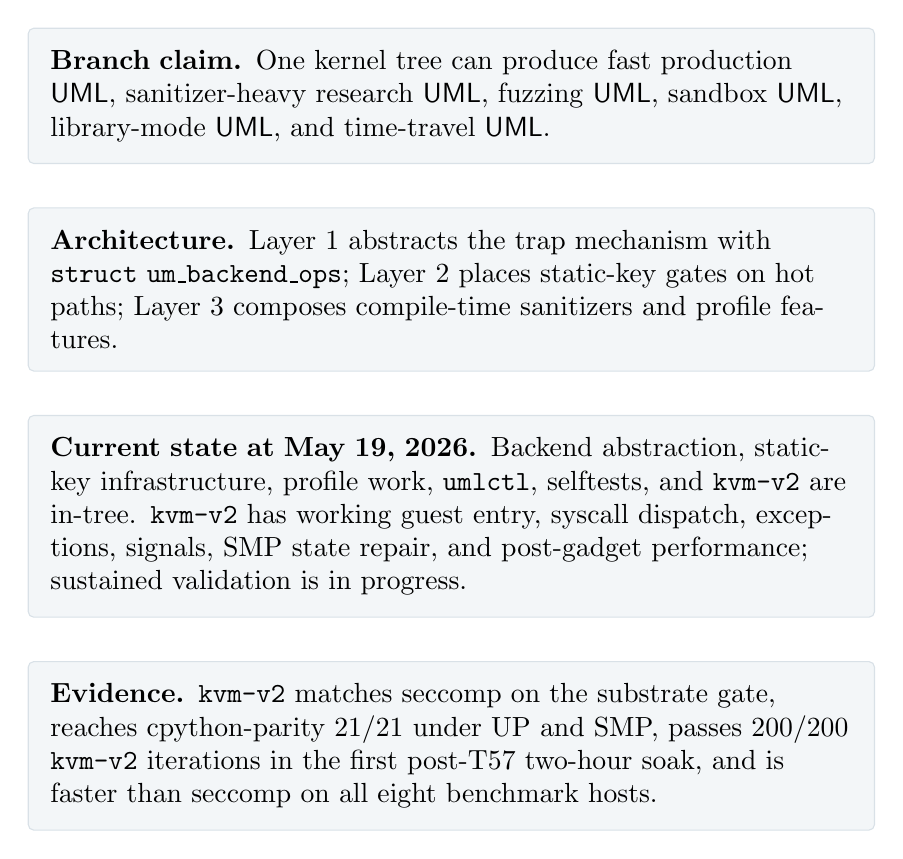
\begin{tikzpicture}[
  node distance=0.55cm,
  box/.style={rounded corners=2pt,draw=UMLGrid,fill=UMLPanel,text width=0.84\textwidth,align=left,inner sep=8pt},
  title/.style={font=\bfseries\large,text=UMLInk},
  key/.style={font=\bfseries,text=UMLBlue},
]
\node[box] (vision) {\textbf{Branch claim.} One kernel tree can produce fast production \UML{}, sanitizer-heavy research \UML{}, fuzzing \UML{}, sandbox \UML{}, library-mode \UML{}, and time-travel \UML{}.};
\node[box,below=of vision] (arch) {\textbf{Architecture.} Layer 1 abstracts the trap mechanism with \texttt{struct um\_backend\_ops}; Layer 2 places static-key gates on hot paths; Layer 3 composes compile-time sanitizers and profile features.};
\node[box,below=of arch] (state) {\textbf{Current state at \ReportDate.} Backend abstraction, static-key infrastructure, profile work, \texttt{umlctl}, selftests, and \KVMvTwo{} are in-tree. \KVMvTwo{} has working guest entry, syscall dispatch, exceptions, signals, SMP state repair, and post-gadget performance; sustained validation is in progress.};
\node[box,below=of state] (evidence) {\textbf{Evidence.} \KVMvTwo{} matches seccomp on the substrate gate, reaches cpython-parity 21/21 under UP and SMP, passes 200/200 \KVMvTwo{} iterations in the first post-T57 two-hour soak, and is faster than seccomp on all eight benchmark hosts.};
\end{tikzpicture}
\caption{The report in four claims. Each claim maps back to a tracked source document or measured artefact.}
\end{figure}

\subsection{Existing UML Contract and Branch Questions}

The branch assumes the existing \UML{} contract: Linux itself runs as a
userspace process, remains debuggable and rootless, and can host
isolated Linux instances without emulating a full machine
\cite{dike-als2000,uml-howto,uml-homepage}. The proposed changes keep
that contract and concentrate on branch-local pressure points:
userspace trap cost, multiprocessor state ownership, profile
composition, and validation breadth.

\begin{table}[h]
\centering
\caption{Existing UML contract mapped to the branch-local response.}
\small
\begin{tabularx}{\linewidth}{@{}L{0.24\linewidth}Y Y@{}}
\toprule
Existing property & Constraint carried forward & Branch-local response \\
\midrule
Kernel as a normal host process & Preserve rootless development, CI usability, and reproducible debugging where nested virtualization is unavailable. & Keep stock-host execution through ptrace/seccomp, but add KVM as a fast backend when available. \\
Isolated Linux instances & Preserve cheap Linux environments without new hardware or privileged host setup. & Make sandbox a profile, not the whole architecture; choose minimal code, seccomp-only defaults, and explicit validation. \\
Faithful upstream kernel & Preserve Linux behavior rather than introducing a userspace reimplementation with semantic drift. & Build the upstream kernel as \UML{}; profiles change defaults and instrumentation, not kernel semantics. \\
Debuggable experimentation & Preserve normal \UML{} debugging value while adding tracing, coverage, and replay hooks as explicit features. & Layer 2 static keys make observability a runtime decision; Layer 3 composes sanitizers by profile. \\
Known hard problems & Treat trap cost and SMP state ownership as implementation and validation problems, not as presentation claims. & \KVMvTwo{} and sustained validation directly target syscall cost, SMP state ownership, parity, and long-run reliability. \\
\bottomrule
\end{tabularx}
\end{table}

\begin{table}[h]
\centering
\caption{Questions the report uses to bound the branch claims.}
\small
\begin{tabularx}{\linewidth}{@{}L{0.04\linewidth}Y Y@{}}
\toprule
\# & Question & Where answered \\
\midrule
1 & What branch-local value proposition is being proposed? & Branch claim, non-goals, existing-contract table, and profile matrix. \\
2 & What is the boundary relative to QEMU, Firecracker, gVisor, LKL, and containers? & Non-goals, design boundary, and adjacent-work comparisons. \\
3 & What single architecture lets fast production, research, fuzzing, sandbox, library, and time-travel coexist? & Three-layer architecture and profile sections. \\
4 & What has actually landed, and what is still only planned? & Current-state tables, source map, and upstream queue. \\
5 & Does \KVMvTwo{} preserve Linux-visible state across SMP, signals, FPU/XSAVE, faults, and task switches? & KVM design, state-audit method, recent-fix table, and validation ladder. \\
6 & Does the performance win survive beyond a microbenchmark? & Micro, Python, and stress-tier benchmark sections. \\
7 & What validation bar remains before upstreaming? & Sustained validation, Tier 2/3/LTP, and next-work sections. \\
8 & What should maintainer review put pressure on next? & Open-state list, remaining risks, and upstream-path sections. \\
\bottomrule
\end{tabularx}
\end{table}

\subsection{Cutoff Snapshot}

\begin{figure}[h]
\centering
\metriccard{UMLBlue}{21/21}{cpython parity\\UP and SMP}\hfill
\metriccard{UMLGreen}{200/200}{\KVMvTwo{} two-hour\\validation pilot}\hfill
\metriccard{UMLAmber}{193--908x}{micro speedup\\over seccomp}\hfill
\metriccard{UMLTeal}{7 series}{staged upstream\\submission queue}
\caption{Dashboard metrics at the reporting cutoff. The numbers are intentionally sparse: each is backed by a source table later in the report.}
\end{figure}

\begin{table}[h]
\centering
\caption{Reporting snapshot.}
\begin{tabularx}{\linewidth}{@{}>{\bfseries}L{0.27\linewidth}Y@{}}
\toprule
Reporting date & \ReportDate \\
Cutoff commit & \texttt{\CutoffCommit} on \texttt{\BranchName} \\
Project corpus & 253 files under \texttt{Documentation/virt/uml/redesign/}; 32 top-level \texttt{tools/testing/selftests/um/} test areas; \texttt{arch/um/backend/kvm-v2/} implementation present \\
Functional headline & \KVMvTwo{} has working guest entry, syscall dispatch, exceptions, signals, SMP state repair, and post-gadget performance; formal 24-hour validation remains open \\
Parity headline & cpython-parity is 21/21 under both UP and SMP; substrate gate is PASS=25/FAIL=3/XFAIL=3, matching seccomp \\
Performance headline & post-gadget \KVMvTwo{} beats seccomp on all eight lab hosts: micro 193--908x, Python 2.99--4.06x, stress 3.71--8.72x \\
Validation headline & first post-T57 two-hour soak: \KVMvTwo{} 200/200 PASS; aggregate 397/400 PASS, with the three failures isolated to iocheck/seccomp timeout behavior \\
\bottomrule
\end{tabularx}
\end{table}

\subsection{What Is Done, What Is Not}

\begin{table}[h]
\centering
\caption{Status by major workstream.}
\begin{tabularx}{\linewidth}{@{}p{0.10\linewidth}p{0.22\linewidth}p{0.18\linewidth}X@{}}
\toprule
ID & Workstream & State & Summary \\
\midrule
A & Backend abstraction & \donepill & \texttt{um\_backend\_ops} contract, ptrace/seccomp split, KUnit contract, and documentation landed. \\
B & Static-key hot paths & \donepill & Hot-path gates, debugfs controls, and runtime flip demonstration landed. \\
C & Profiles and gaps & \statuspill{UMLGreen}{MOSTLY} & Defconfigs and major sanitizer/tracing ports are largely landed; snapshot, syzkaller, and some resumed features remain. \\
D & KVM backend & \progresspill & \KVMvTwo{} is functional and performant; 24-hour validation, Tier 2/3, LTP, and upstream packaging are the active edge. \\
\bottomrule
\end{tabularx}
\end{table}

\subsection{First Three-Page Takeaway}

The branch is best understood as a transition from one default
execution story to an explicit profile matrix. The common lower layer
is a backend contract; production can choose \KVM{}, CI can choose
\Seccomp{}, legacy hosts can choose ptrace, and each profile can decide
whether it wants no hooks, runtime hooks, or heavy compile-time
instrumentation.

The current branch has crossed the highest-risk implementation path:
\KVMvTwo{} can run real guest userspace, handle SMP, preserve
cross-task state, and beat \Seccomp{} on measured workloads. The
remaining gate is sustained validation: reliability, breadth, and
upstreamable series boundaries.


\newpage
\tableofcontents
\newpage

\section{Goal and Vision}

\subsection{Problem Statement}

Classic \UML{} remains valuable because it is Linux itself compiled
to run as a userspace program. That gives researchers a real kernel,
real system call semantics, and a deployable target in environments
where full hardware virtualization is not available. The problem is
that the historical execution model does not provide the performance,
feature composition, or operational discipline expected by modern
kernel fuzzing and observability workflows.

The redesign sets a higher bar:
\begin{itemize}
  \item production \UML{} should approach native syscall cost when
        the host exposes \KVM{};
  \item research \UML{} should ship with sanitizers, tracing,
        kprobes, ftrace, BPF, KGDB, and debug surfaces composed from
        one tree;
  \item fuzzing \UML{} should provide KCOV, snapshot/forkserver
        startup, and a path toward a syzkaller \texttt{vm/uml}
        backend;
  \item sandbox \UML{} should compile out debug surfaces and minimize
        host attack surface;
  \item time-travel and record/replay should become a profile, not a
        niche configuration footnote.
\end{itemize}

\subsection{Non-Goals}

The design deliberately avoids three tempting but wrong shapes.
First, it does not reimplement Linux in another language. gVisor is
important prior art for backend structure and \KVM{} execution, but
\UML{} keeps Linux semantics by building Linux itself
\cite{gvisor-platforms}. Second, it is not a microVM competitor to
Firecracker \cite{firecracker}; the problem is kernel research and
fuzzing fidelity, not cloud cold-start packaging. Third, it is not a
unikernel-only library effort, although the library profile borrows
from LKL where that model is useful \cite{lkl}.

\subsection{Success Criteria}

The project succeeds when a developer can select a profile, build it
from the same tree, and get an artifact whose performance and
instrumentation properties match its intended use:

\begin{table}[h]
\centering
\caption{Target profile outcomes.}
\begin{tabularx}{\linewidth}{@{}p{0.21\linewidth}X@{}}
\toprule
Profile & Intended outcome \\
\midrule
\texttt{prod-fast} & \KVM{} backend, no hooks, near-native syscall path. \\
\texttt{prod-with-hooks} & Fast production binary with hooks compiled but off; tracing can be enabled after a crash without rebuilding. \\
\texttt{research} & Debug-friendly \UML{} with tracing, kprobes, sanitizers, and interactive control surfaces. \\
\texttt{fuzz} / \texttt{fuzz-deep} & KCOV, snapshots, sanitizer coverage, replay-oriented hooks, and syzkaller integration. \\
\texttt{sandbox} & Minimal debug surface and minimized host-side trust boundary. \\
\texttt{library} & LKL-style direct-call mode for harnesses that can sacrifice ring-split fidelity. \\
\texttt{time-travel} & Deterministic time and replay hooks as a first-class shipped configuration. \\
\bottomrule
\end{tabularx}
\end{table}

\subsection{Why Now}

The timing is favorable because recent \UML{} work removed old
prerequisite blockers: seccomp mode exists, SMP support exists, and
modern kernel instrumentation is mature enough to compose around
static keys and profile-specific Kconfig. The surrounding ecosystem
also supplies useful models: gVisor for backend/platform design,
crosvm for host process decomposition \cite{crosvm}, syzkaller for
fuzzing expectations \cite{syzkaller}, and upstream kernel policy for
AI-assisted development disclosure \cite{coding-assistants}.

\section{Current State}

\subsection{Source Basis}

The report is grounded in the branch's source material: goal and plan
documents, landed code, the bug diary, current status, and measured
evidence. The main source classes are:

\begin{table}[h]
\centering
\caption{How the project corpus maps into this report.}
\small
\begin{tabularx}{\linewidth}{@{}L{0.16\linewidth}L{0.33\linewidth}Y@{}}
\toprule
Source class & Representative paths & Use in the report \\
\midrule
Plan and vision & \path{00-vision.md}, \path{README.md}, \path{report-presentation/PLAN.md} & Defines the goal, non-goals, architecture narrative, and publishing shape. \\
Architecture & \path{01-architecture/}, \path{02-workstreams/} & Defines layers, workstreams, dependencies, profiles, and sequencing. \\
Code & \path{arch/um/include/shared/backend.h}, \path{arch/um/backend/kvm-v2/}, \path{tools/uml/uml-launcher/} & Confirms that the report is describing landed implementation, not only design. \\
Diary and state & \path{STATUS.md}, \path{state-audit/}, sustained-validation memos & Provides current truth, bug chronology, closure criteria, and remaining work. \\
Evidence & \path{tools/testing/selftests/um/}, benchmark and soak memos & Supplies measured performance, parity, soak, and gate data. \\
\bottomrule
\end{tabularx}
\end{table}

\subsection{Inherited \UML{} Versus This Branch}

The attribution boundary matters. I checked it by diffing
\texttt{origin/master...HEAD} across \texttt{arch/um},
\texttt{tools/uml}, \texttt{tools/testing/selftests/um}, and
\texttt{Documentation/virt/uml}. That diff spans 688 UML-related
files, with 154,501 insertions and 823 deletions. The number is a
scope check, not an authorship claim: the existing \UML{} model, the
Linux kernel, and generic \KVM{} facilities remain inherited foundations.

\begin{table}[h]
\centering
\caption{Attribution boundary for the current branch.}
\small
\begin{tabularx}{\linewidth}{@{}L{0.24\linewidth}Y@{}}
\toprule
Category & What the report means \\
\midrule
Inherited \UML{} and Linux & Linux-as-a-host-process, the upstream
\UML{} port, legacy ptrace execution, existing kernel subsystems,
the host KVM API, and the general idea of deterministic time-travel
are not claimed as new work here. \\
Recent upstream prerequisites & Seccomp-mode \UML{} and upstream
SMP work are treated as enabling context. The redesign builds on
them; it does not present them as branch-local inventions. \\
Redesigned in this project & The explicit backend-ops contract,
static-key hook model, profile matrix, validation ladder, staged
upstream queue, and \KVMvTwo{} state-ownership method are the project
architecture. \\
Implemented in this branch & \path{arch/um/backend/kvm-v2/},
backend contract code, profile configs and docs, snapshot/forkserver
v1, the Rust launcher and \texttt{umlctl}, KVM/soak/benchmark
selftests, and the report/deck workspace are branch-local artefacts. \\
Planned or paused & KVM-aware snapshot readiness, full record/replay,
time-machine workflow, syzkaller \texttt{vm/uml}, LTP curation, and
the large upstream \texttt{arch/um} series remain future work. \\
\bottomrule
\end{tabularx}
\end{table}

\subsection{Landed Versus Open}

The branch contains substantial code and test infrastructure:

\begin{itemize}
  \item \texttt{arch/um/include/shared/backend.h} defines the backend
        contract used by host-side and kernel-side translation units.
  \item \texttt{arch/um/backend/seccomp/} and ptrace integration
        provide the non-\KVM{} backends.
  \item \texttt{arch/um/backend/kvm-v2/} contains the active \KVMvTwo{}
        implementation, including vCPU, memory, syscall, exception,
        region, state trace, and LSTAR gadget code.
  \item \texttt{tools/uml/uml-launcher/} and \texttt{umlctl} provide
        host-side launch, supervision, gate, gate-loop, history, and
        deployment machinery.
  \item \texttt{tools/testing/selftests/um/} contains benchmark,
        parity, gate, soak, snapshot, KVM, ftrace, kprobes, KMSAN, and
        process reproducer coverage.
\end{itemize}

\begin{figure}[h]
\centering
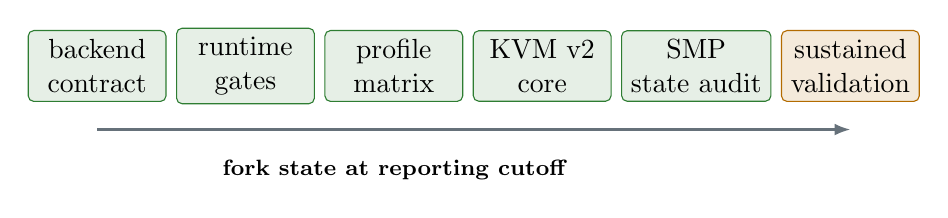
\begin{tikzpicture}[
  lane/.style={draw=UMLGrid,fill=UMLPanel,rounded corners=2pt,minimum height=0.75cm,align=center},
  done/.style={draw=UMLGreen,fill=UMLGreen!12},
  prog/.style={draw=UMLAmber,fill=UMLAmber!14},
  label/.style={font=\footnotesize\bfseries},
]
\node[lane,done,minimum width=1.75cm] (a) {backend\\contract};
\node[lane,done,minimum width=1.75cm,right=0.12cm of a] (b) {runtime\\gates};
\node[lane,done,minimum width=1.75cm,right=0.12cm of b] (c) {profile\\matrix};
\node[lane,done,minimum width=1.75cm,right=0.12cm of c] (d) {KVM v2\\core};
\node[lane,done,minimum width=1.75cm,right=0.12cm of d] (g) {SMP\\state audit};
\node[lane,prog,minimum width=1.75cm,right=0.12cm of g] (j) {sustained\\validation};
\draw[-{Latex[length=2mm]},thick,UMLMuted] (a.south) ++(0,-0.35) -- ($(j.south)+(0,-0.35)$);
\node[label,below=0.62cm of c] {fork state at reporting cutoff};
\end{tikzpicture}
\caption{High-level milestone state. Most architectural and implementation work has landed; sustained validation is the active formal gate.}
\end{figure}

\subsection{Current Functional Reading}

\begin{table}[h]
\centering
\caption{Functional status from \texttt{STATUS.md}.}
\begin{tabularx}{\linewidth}{@{}L{0.31\linewidth}L{0.19\linewidth}Y@{}}
\toprule
Surface & Reading & Interpretation \\
\midrule
\texttt{init=/bin/echo} & UP + SMP yes & Basic guest entry works under \KVMvTwo{}. \\
Python smoke & UP + SMP yes & \texttt{python3 -V}, hashlib, ssl, and single imports work. \\
Substrate gate & PASS=25, FAIL=3, XFAIL=3 & \KVMvTwo{} matches \Seccomp{} on the curated substrate gate. \\
cpython-parity & 21/21 & The old P0, Python C-extension import crashes, is functionally closed. \\
mt-mini T=8, ncpus=4 & 30/30 or better in current runs & SMP memory stress reaches the current acceptance bar. \\
threaded-fork-malloc & 0/24000 child failures & Cross-task XMM/FPU guarantee survived the T55/T57 fixes. \\
wide cpython-parity & 134 parity, 0 regression & Larger curated module sweep found no \KVMvTwo{} regression. \\
\bottomrule
\end{tabularx}
\end{table}

\subsection{Open State}

The important open items are bounded:
\begin{itemize}
  \item Sustained validation must still deliver a formal 24-hour continuous run,
        Tier 2/Tier 3 workload templates, and LTP curation.
  \item Snapshot and record/replay work is unblocked but paused behind
        sustained validation.
  \item The T57 AVX/XSAVE fix is landed; AVX-512 exposure is
        deferred to a follow-up if needed.
  \item The LKML queue is sequenced, but the large \texttt{arch/um}
        series are gated on validation and upstream review strategy.
\end{itemize}

\section{Architecture}

\subsection{Three Layers}

\begin{figure}[h]
\centering
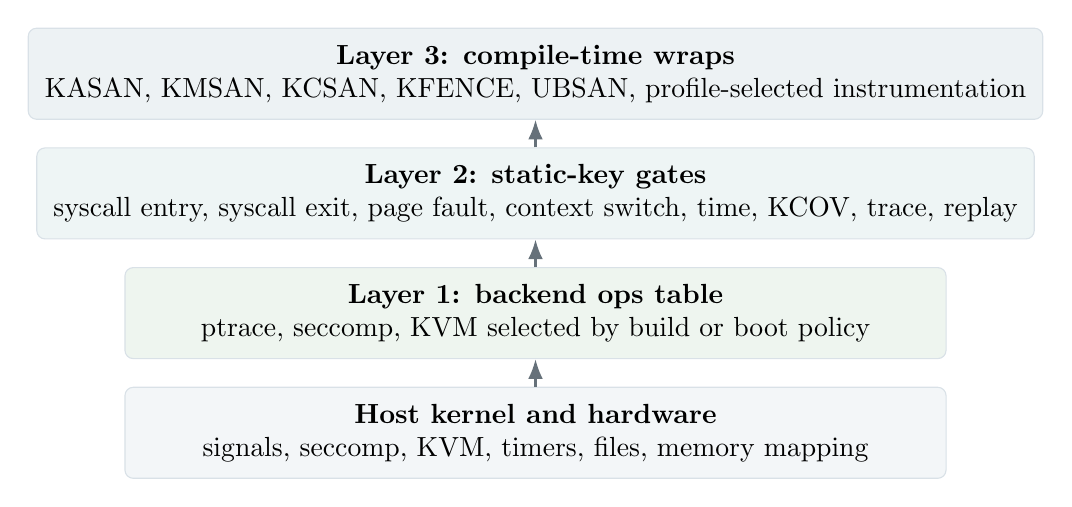
\begin{tikzpicture}[
  layer/.style={draw=UMLGrid,rounded corners=3pt,minimum width=0.86\linewidth,minimum height=1.1cm,align=center,inner sep=6pt},
  arrow/.style={-{Latex[length=2.5mm]},thick,UMLMuted},
]
\node[layer,fill=UMLBlue!8] (l3) {\textbf{Layer 3: compile-time wraps}\\KASAN, KMSAN, KCSAN, KFENCE, UBSAN, profile-selected instrumentation};
\node[layer,fill=UMLTeal!8,below=0.35cm of l3] (l2) {\textbf{Layer 2: static-key gates}\\syscall entry, syscall exit, page fault, context switch, time, KCOV, trace, replay};
\node[layer,fill=UMLGreen!8,below=0.35cm of l2] (l1) {\textbf{Layer 1: backend ops table}\\ptrace, seccomp, KVM selected by build or boot policy};
\node[layer,fill=UMLPanel,below=0.35cm of l1] (host) {\textbf{Host kernel and hardware}\\signals, seccomp, KVM, timers, files, memory mapping};
\draw[arrow] (host) -- (l1);
\draw[arrow] (l1) -- (l2);
\draw[arrow] (l2) -- (l3);
\end{tikzpicture}
\caption{The architectural decomposition. Lower layers do not know about higher-layer policy; profiles choose points in the product space.}
\end{figure}

Layer 1 isolates the mechanism that makes guest userspace run:
ptrace, \Seccomp{}, or \KVM{}. Layer 2 isolates optional runtime
observation and policy hooks. Layer 3 isolates compiler-level
instrumentation whose cost is inherent in the binary. This structure
matches the host kernel's own composition strategy: explicit lower
interfaces, static keys for runtime feature toggles, and Kconfig for
compile-time feature selection.

\subsection{Layer 1: Backend Contract}

The live contract is \texttt{struct um\_backend\_ops}. It has
metadata, capability flags, lifecycle hooks, vCPU execution, memory
region callbacks, scheduling hooks, TLB kick support, time hooks, and
debug/introspection hooks. The important design choices are:

\begin{itemize}
  \item every in-tree backend populates the whole table; unsupported
        cold operations return an explicit error rather than leaving
        NULL fields;
  \item single-backend builds can compile calls down to direct calls;
        dynamic builds can select at boot and pay one stable indirect
        call;
  \item backend capability flags replaced legacy global booleans, so
        host-side code asks the selected backend what stub, reaper, and
        syscall behavior it needs;
  \item per-mm memory state is owned by the backend, which lets
        \Seccomp{} keep its stub model while \KVMvTwo{} manages
        memslots and guest mappings.
\end{itemize}

\begin{table}[h]
\centering
\caption{Backend contract categories.}
\begin{tabularx}{\linewidth}{@{}p{0.2\linewidth}p{0.19\linewidth}X@{}}
\toprule
Category & Representative ops & Why it belongs in Layer 1 \\
\midrule
Lifecycle/trap & \texttt{probe}, \texttt{init}, \texttt{vcpu\_run} & Backend availability and guest execution are mechanism-specific. \\
Memory & \texttt{mm\_create}, region add, remove, protect & ptrace/seccomp stubs and \KVM{} memslots have different state models. \\
Scheduling & thread create, context switch, IPI & Guest scheduling touches backend-owned vCPU or stub state. \\
Time & clock read, timer set & Determinism and backend timing sources must be abstracted. \\
Debug & register read/write & KGDB and inspection need a common contract over different mechanisms. \\
\bottomrule
\end{tabularx}
\end{table}

\subsection{Layer 2: Static-Key Hot Paths}

Layer 2 is the answer to a central tension: a research build wants
hooks everywhere; a production build wants the hot path cold and
small. Static keys make the disabled case a patched NOP sequence and
the enabled case an explicit branch to slow-path code. The off-state
cost model is therefore stable and auditable.

The report treats Layer 2 as a policy plane rather than a pile of
tracepoints. The same hot path can support tracing, KCOV,
record/replay, time-travel, and performance event emission, provided
each hook has a clear default state and each profile declares which
hooks are compiled and enabled.

\subsection{Layer 3: Compile-Time Instrumentation}

Layer 3 includes KASAN, KMSAN, KCSAN, KFENCE, UBSAN, and related
compiler- or allocator-level instrumentation. These features cannot be
made free by a runtime branch. They change code generation, memory
layout, or allocator behavior. The architecture therefore treats them
as profile-level build choices that compose with any backend below.

\subsection{A Syscall Through the Stack}

\begin{figure}[h]
\centering
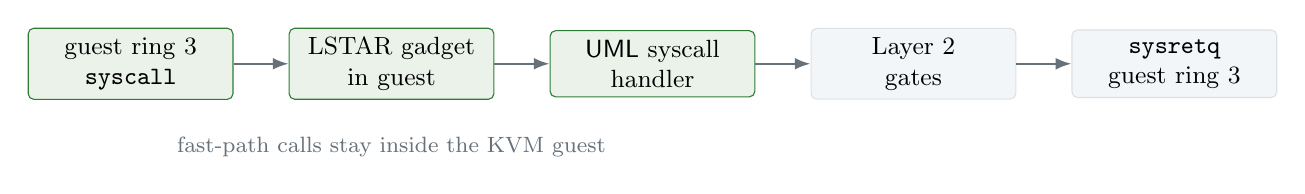
\begin{tikzpicture}[
  flowstep/.style={draw=UMLGrid,fill=UMLPanel,rounded corners=2pt,minimum width=2.6cm,minimum height=0.8cm,align=center,font=\small},
  fast/.style={draw=UMLGreen,fill=UMLGreen!10},
  slow/.style={draw=UMLAmber,fill=UMLAmber!12},
  arr/.style={-{Latex[length=2mm]},thick,UMLMuted},
]
\node[flowstep,fast] (u) {guest ring 3\\\texttt{syscall}};
\node[flowstep,fast,right=0.7cm of u] (gadget) {LSTAR gadget\\in guest};
\node[flowstep,fast,right=0.7cm of gadget] (kernel) {\UML{} syscall\\handler};
\node[flowstep,right=0.7cm of kernel] (gates) {Layer 2\\gates};
\node[flowstep,right=0.7cm of gates] (ret) {\texttt{sysretq}\\guest ring 3};
\draw[arr] (u) -- (gadget);
\draw[arr] (gadget) -- (kernel);
\draw[arr] (kernel) -- (gates);
\draw[arr] (gates) -- (ret);
\node[below=0.35cm of gadget,font=\footnotesize,text=UMLMuted] {fast-path calls stay inside the KVM guest};
\end{tikzpicture}
\caption{\KVMvTwo{} fast syscall shape after gadget revival. Trivial syscalls avoid a host vmexit on the hot path.}
\end{figure}

\section{KVM v2 Design}

\subsection{Model}

\KVMvTwo{} follows the gVisor KVM-platform idea, adapted to \UML{}:
guest userspace runs at ring 3 inside a KVM guest, the \UML{} kernel
runs at ring 0 inside the same KVM guest, and ordinary syscalls enter
the \UML{} kernel through MSR\_LSTAR instead of trapping to a host
monitor \cite{gvisor-platforms,kvm-api}. Host exits are still used for
operations that truly require host participation, but the target is
to keep the common syscall path in guest context.

\begin{figure}[h]
\centering
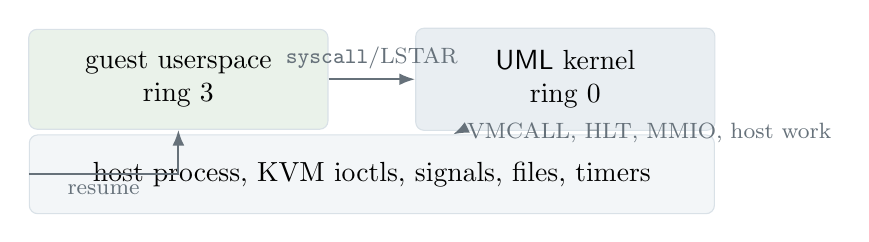
\begin{tikzpicture}[
  region/.style={draw=UMLGrid,rounded corners=3pt,align=center,inner sep=8pt},
  arr/.style={-{Latex[length=2mm]},thick,UMLMuted},
]
\node[region,fill=UMLGreen!10,minimum width=3.8cm,minimum height=1.25cm] (user) {guest userspace\\ring 3};
\node[region,fill=UMLBlue!10,minimum width=3.8cm,minimum height=1.25cm,right=1.1cm of user] (kernel) {\UML{} kernel\\ring 0};
\node[region,fill=UMLPanel,minimum width=8.7cm,minimum height=1.0cm,below=0.7cm of $(user)!0.5!(kernel)$] (host) {host process, KVM ioctls, signals, files, timers};
\draw[arr] (user) -- node[above,font=\footnotesize]{\texttt{syscall}/LSTAR} (kernel);
\draw[arr] (kernel) -- node[right,font=\footnotesize]{VMCALL, HLT, MMIO, host work} (host);
\draw[arr] (host) -| node[pos=0.25,below,font=\footnotesize]{resume} (user);
\end{tikzpicture}
\caption{\KVMvTwo{} execution model. It is not a QEMU-style machine; it is a trap mechanism for \UML{} itself.}
\end{figure}

\subsection{Implementation Themes}

The current \KVMvTwo{} design is organized around five hard problems:

\begin{enumerate}
  \item \textbf{Guest entry and return.} The backend must enter guest
        ring 3, handle SYSCALL/SYSRET transitions, and recover when
        host signals interrupt critical regions.
  \item \textbf{Per-vCPU and per-task state.} General registers,
        CR2, segment bases, FPU/XSAVE, pending events, IST frames,
        and KVM run state cannot leak across tasks or host CPUs.
  \item \textbf{Memory and TLB state.} \UML{} page-table changes must
        be reflected into KVM-visible mappings and cross-vCPU TLB
        state without stale translations.
  \item \textbf{SMP correctness.} Host scheduling, guest scheduling,
        signal delivery, and KVM vCPU ownership must compose without
        assuming that \texttt{preempt\_disable()} pins a host thread.
  \item \textbf{Performance.} The backend must preserve the win from
        in-guest dispatch while avoiding correctness regressions from
        lazy state handling.
\end{enumerate}

\subsection{Design Detail: Main Control Surfaces}

\begin{table}[h]
\centering
\caption{\KVMvTwo{} implementation surfaces to understand before reviewing patches.}
\small
\begin{tabularx}{\linewidth}{@{}L{0.21\linewidth}L{0.29\linewidth}Y@{}}
\toprule
Surface & Representative code & Design role \\
\midrule
Initialization and capabilities & \path{init.c}, \path{ops.c}, \path{Kconfig} & Probe host KVM support, wire backend ops, expose configuration choices. \\
vCPU execution & \path{vcpu.c} & Owns KVM\_RUN, register marshaling, migration pinning, FPU capture, dispatch, and per-vCPU state. \\
Syscall path & \path{syscall_trap.c}, \path{lstar_gadget.S} & Handles LSTAR entry, in-guest fast syscalls, slow-path exits, and return-state repair. \\
Memory and regions & \path{memslot.c}, \path{region.c}, backend memory ops & Maps \UML{} memory changes into KVM-visible regions and memslot policy. \\
Exceptions & \path{exception.c} & Installs and handles IDT/TSS/IST paths, page faults, and special recovery paths. \\
State tracing & \path{state_trace.[ch]} & Gives low-overhead, static-key-controlled visibility into state ownership bugs. \\
Tests & \path{test_marshal.c}, \path{test_byteshape.c} & Protect register ABI, gadget byte shape, and internal assumptions. \\
\bottomrule
\end{tabularx}
\end{table}

\subsection{Design Detail: Fast Path Versus Slow Path}

The backend now has two different syscall cost classes. Trivial
syscalls covered by the LSTAR gadget stay inside the KVM guest and
return directly to guest userspace. Syscalls outside the gadget set,
or paths requiring host assistance, still exit to the host and run the
full backend machinery. The project should keep these paths described
separately:

\begin{itemize}
  \item \textbf{Fast path:} getpid-family and clock-like calls that
        can be answered from guest-visible state with preserved ABI
        registers and no host-side work.
  \item \textbf{Slow path:} mmap, munmap, brk, I/O, scheduling,
        signal, and fault paths that need backend state or host
        services.
  \item \textbf{Recovery path:} interrupted LSTAR, page-fault stub,
        \#NM, and signal delivery edges where the backend must rebuild
        user-visible architectural state exactly.
\end{itemize}

\subsection{State-Audit Method}

The state-audit directory is part of the design, not just project
diary. It converted a vague SMP corruption class into a finite audit:
149 state items, 50+ operations, an ownership matrix, suspect
register audits, runtime tracing, and ranked findings.

\begin{table}[h]
\centering
\caption{State-audit layers.}
\begin{tabularx}{\linewidth}{@{}p{0.09\linewidth}p{0.29\linewidth}X@{}}
\toprule
Layer & Artefact & Contribution \\
\midrule
1 & State inventory & Enumerates register, control, segment, MSR, FPU, event, descriptor, per-task, per-vCPU, and per-mm state. \\
2 & Operations inventory & Lists hardware, KVM, backend, scheduler, and signal operations that read or write state. \\
3 & Ownership matrix & States who owns each state item at each transition. \\
4 & Suspect register audits & Tracks RBP, RAX, RDX, FS\_BASE and similar corruption signatures. \\
5 & Toolkit & cscope, ripgrep, ast-grep, bpftrace, ftrace, and parser recipes. \\
6--8 & Findings and fixes & Converts candidates into patches and regression matrices. \\
\bottomrule
\end{tabularx}
\end{table}

The most important fix from this arc was the SMP-T13
\texttt{migrate\_disable()} finding. \UML{} was using
\texttt{preempt\_disable()} to pin access to per-host-CPU vCPU state,
but the build did not have preemption count semantics, so the call did
not actually prevent migration. Replacing that assumption with
\texttt{migrate\_disable()} removed a structural cross-vCPU ownership
violation.

\subsection{Recent Fixes}

\begin{table}[h]
\centering
\caption{Selected recent \KVMvTwo{} correctness and performance closures.}
\begin{tabularx}{\linewidth}{@{}p{0.17\linewidth}p{0.25\linewidth}X@{}}
\toprule
Item & Closure & Why it matters \\
\midrule
SMP-T41 & Recover user RAX in EINTR-mid-PF-stub & Closed the true mt-mini byte-zero residual. \\
SMP-T54 & SOCK\_CLOEXEC and \texttt{umlctl} sysrq halt & Removed worker fd leak and init shutdown hang class. \\
SMP-T55 & Per-vCPU FPU-dirty epoch & Restored perf-py-startup gate while preserving cross-task FPU guarantees. \\
SMP-T57 Phase A & CR4.OSXSAVE, XCR0=0x7, CPUID AVX/XSAVE unmask & Turned stress-ng AVX \#UD from a fragile mask problem into supported guest architectural state. \\
Gadget revival & LSTAR in-guest fast path & Collapsed trivial syscall cost from host-exit scale to roughly 90 cycles on measured hosts. \\
\bottomrule
\end{tabularx}
\end{table}

\subsection{Design Boundary}

The current backend should be presented upstream as a backend for
\UML{}, not as a general VMM. The VMM-like machinery exists only to
make \UML{} execution fast and faithful. That framing matters: it
keeps device emulation, boot firmware, hardware discovery, and cloud
microVM expectations out of scope.

\section{Profiles and Validation}

\subsection{Profile Matrix}

\begin{table}[h]
\centering
\caption{Shipped profile intent.}
\small
\begin{tabularx}{\linewidth}{@{}p{0.17\linewidth}p{0.18\linewidth}p{0.22\linewidth}p{0.17\linewidth}X@{}}
\toprule
Profile & Backend default & Hooks & Sanitizers & Purpose \\
\midrule
\texttt{prod-fast} & KVM $>$ seccomp & none & none & Minimum overhead production target. \\
\texttt{prod-with-hooks} & KVM $>$ seccomp & compiled, off & none & Production artifact with post-failure observability. \\
\texttt{research} & seccomp & trace, kprobes & KASAN, UBSAN & Debug and exploit-reproduction profile. \\
\texttt{fuzz} & seccomp & KCOV, snapshot & KASAN & syzkaller and harness fuzzing. \\
\texttt{fuzz-deep} & seccomp & KCOV, snapshot, replay & KASAN, KCSAN & deeper race/replay investigations. \\
\texttt{sandbox} & seccomp-only & none compiled & none & Minimized TCB and debug surface. \\
\texttt{library} & direct call & n/a & optional KASAN & LKL-style harness integration. \\
\texttt{embedded} & ptrace & none & none & Old-host fallback. \\
\texttt{time-travel} & seccomp & trace, time-travel & KASAN & deterministic clock and replay. \\
\bottomrule
\end{tabularx}
\end{table}

\begin{figure}[h]
\centering
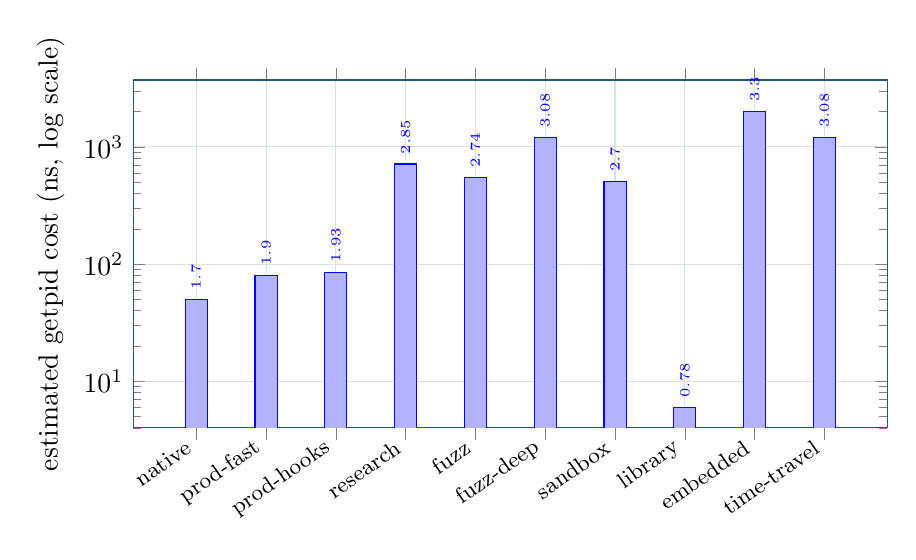
\begin{tikzpicture}
\begin{axis}[
  width=0.92\linewidth,
  height=6.0cm,
  ybar,
  ymode=log,
  log basis y=10,
  ymin=4,
  ylabel={estimated getpid cost (ns, log scale)},
  symbolic x coords={native,prod-fast,prod-hooks,research,fuzz,fuzz-deep,sandbox,library,embedded,time-travel},
  xtick=data,
  xticklabel style={rotate=35,anchor=east,font=\footnotesize},
  bar width=8pt,
  fill=UMLBlue!70,
  draw=UMLBlue,
  nodes near coords,
  nodes near coords style={font=\tiny,rotate=90,anchor=west},
  grid=major,
  major grid style={draw=UMLGrid},
]
\addplot coordinates {
  (native,50) (prod-fast,80) (prod-hooks,85) (research,715) (fuzz,550)
  (fuzz-deep,1200) (sandbox,505) (library,6) (embedded,2000)
  (time-travel,1200)
};
\end{axis}
\end{tikzpicture}
\caption{Profile cost model from the redesign docs, anchored to a 50 ns normal Linux \texttt{getpid} baseline. The value of profiles is the ability to span direct-call library mode through heavily instrumented research and time-travel builds without forking the tree.}
\end{figure}

\subsection{Validation Ladder}

\begin{figure}[h]
\centering
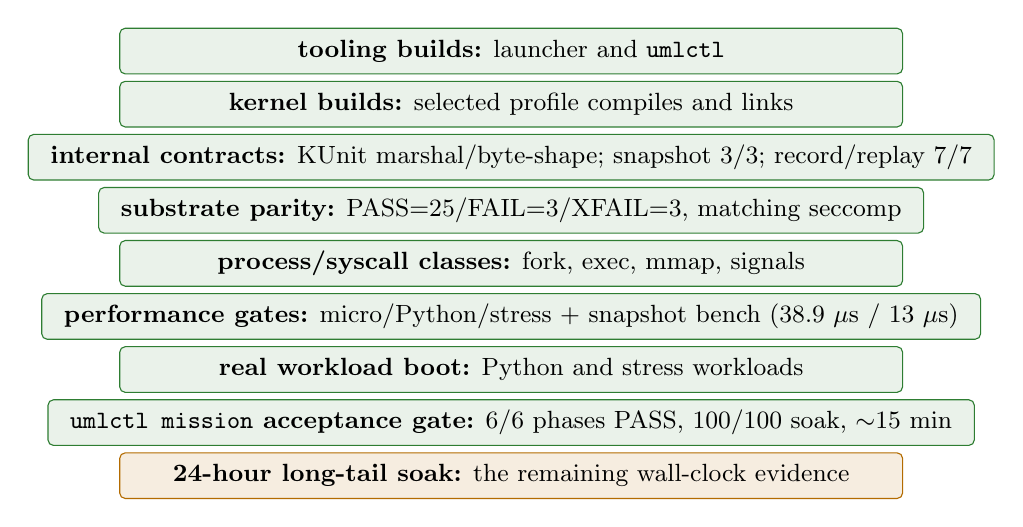
\begin{tikzpicture}[
  rung/.style={draw=UMLGrid,fill=UMLPanel,rounded corners=2pt,minimum width=0.82\linewidth,minimum height=0.58cm,align=left,inner xsep=8pt,font=\small},
  live/.style={draw=UMLGreen,fill=UMLGreen!10},
  prog/.style={draw=UMLAmber,fill=UMLAmber!12},
]
\node[rung,live] (l0) {\textbf{tooling builds:} launcher and \texttt{umlctl}};
\node[rung,live,below=0.08cm of l0] (l1) {\textbf{kernel builds:} selected profile compiles and links};
\node[rung,live,below=0.08cm of l1] (l2) {\textbf{internal contracts:} KUnit marshal/byte-shape; snapshot 3/3; record/replay 7/7};
\node[rung,live,below=0.08cm of l2] (l3) {\textbf{substrate parity:} PASS=25/FAIL=3/XFAIL=3, matching seccomp};
\node[rung,live,below=0.08cm of l3] (l4) {\textbf{process/syscall classes:} fork, exec, mmap, signals};
\node[rung,live,below=0.08cm of l4] (l5) {\textbf{performance gates:} micro/Python/stress + snapshot bench (38.9~$\mu$s / 13~$\mu$s)};
\node[rung,live,below=0.08cm of l5] (l6) {\textbf{real workload boot:} Python and stress workloads};
\node[rung,live,below=0.08cm of l6] (l7) {\textbf{\texttt{umlctl mission} acceptance gate:} 6/6 phases PASS, 100/100 soak, $\sim$15 min};
\node[rung,prog,below=0.08cm of l7] (l8) {\textbf{24-hour long-tail soak:} the remaining wall-clock evidence};
\end{tikzpicture}
\caption{Validation ladder. Short gates protect the inner loop; the \texttt{umlctl mission} acceptance gate is the single-binary verdict; sustained 24-hour validation is the long-tail evidence reserved for milestone candidates.}
\end{figure}

\subsection{\texttt{umlctl mission} Acceptance Gate (2026-05-19)}

The first-class \texttt{umlctl mission} command replaces the
ad-hoc soak invocation. One command, six fail-fast phases, a
binary verdict, and a JSON scoreboard. Total wall-clock is
$\sim$15 min including an 8-min diverse-workload soak.

\begin{table}[h]
\centering
\caption{Mission-accomplished run, kernel \texttt{9ccbf5e7bb58}, host server7, 2026-05-19.}
\small
\begin{tabularx}{\linewidth}{@{}p{0.04\linewidth}p{0.16\linewidth}p{0.10\linewidth}p{0.10\linewidth}X@{}}
\toprule
\# & Phase & Verdict & Duration & Summary \\
\midrule
1 & KUnit & \donepill & 5.0~s & 10/10 cases PASS (snapshot 3 + record 7) \\
2 & Bench & \donepill & 2.5~s & capture 35~$\mu$s, median restore 13~$\mu$s (targets <50~ms / <1~ms) \\
3 & Substrate & \donepill & 3.5~s & cpython-tier0 PASS \\
4 & Host resources & \donepill & 1.4~s & UM\_THP / UM\_OOM\_SCORE\_ADJ / UM\_KVM\_V2\_CPU\_AFFINITY applied silently; backend banner clean \\
5 & Diverse soak & \donepill & 855.0~s & 100/100 PASS across memcheck + iocheck + stress-ng + tier1-pylibs + django-loopback-none; 0 panics / 0 SIGBUS / 0 high-cr2 \\
6 & Diagnostic & \donepill & 0.4~s & kernel SHA-256, host, hugepage pool sizing, cgroup v2 state captured \\
\midrule
\multicolumn{2}{@{}l}{\textbf{MISSION\_ACCOMPLISHED}} & \multicolumn{3}{l}{867.7~s total wall-clock (14.5~min)} \\
\bottomrule
\end{tabularx}
\end{table}

The mission gate is designed so a \emph{single} regression in any
phase --- a flipped KUnit case, a missed performance target, a
substrate gate break, an env-var-knob malfunction, a panic during
soak, or a misconfigured host that the preflight catches ---
produces \texttt{MISSION\_FAILED phase=<N>} on stderr and a
non-zero exit. The Phase 5 gate explicitly fails on any of
panics, ``Kernel mode signal 7'' (/dev/shm exhaustion), or
``high-cr2'' (the residual user-fault flake class) regardless of
the aggregate pass rate.

\subsection{Earlier Sustained Validation Pilot (2026-05-14)}

The first post-T57 short pilot remains in the record as the
chronological predecessor of the mission gate:

\begin{table}[h]
\centering
\caption{First post-T57 sustained-validation pilot, 2026-05-14, retained for chronology.}
\small
\begin{tabular}{@{}llrrrr@{}}
\toprule
Workload & Backend & n & pass & fail & pass rate \\
\midrule
memcheck & \KVMvTwo{} & 60 & 60 & 0 & 100.00\% \\
memcheck & seccomp & 60 & 60 & 0 & 100.00\% \\
iocheck & \KVMvTwo{} & 60 & 60 & 0 & 100.00\% \\
iocheck & seccomp & 60 & 57 & 3 & 95.00\% \\
stress-ng & \KVMvTwo{} & 40 & 40 & 0 & 100.00\% \\
stress-ng & seccomp & 40 & 40 & 0 & 100.00\% \\
tier1-pylibs & \KVMvTwo{} & 40 & 40 & 0 & 100.00\% \\
tier1-pylibs & seccomp & 40 & 40 & 0 & 100.00\% \\
\midrule
\multicolumn{2}{@{}l}{\textbf{\KVMvTwo{} aggregate}} & 200 & 200 & 0 & \textbf{100.00\%} \\
\multicolumn{2}{@{}l}{\textbf{Overall aggregate}} & 400 & 397 & 3 & \textbf{99.25\%} \\
\bottomrule
\end{tabular}
\end{table}

This pilot validated daemon mode, threshold-trip behaviour,
Wilson summary generation, and sustained \KVMvTwo{} workload
rotation. The three failures were iocheck/seccomp timeout shape,
not \KVMvTwo{} regressions. The \texttt{umlctl mission} gate
above subsumes this pilot as the canonical acceptance artefact.

\section{Performance and Benchmarks}

\subsection{Benchmark Method}

The post-gadget cross-host benchmark used one kernel build, one
benchmark bundle, the same orchestrator, performance governor, and the
same three tiers across eight lab hosts:
\begin{itemize}
  \item \textbf{micro}: \texttt{getpid-loop}, RDTSC-bracketed, pure
        trap-mechanism cost.
  \item \textbf{py}: canned Python startup/mixed-syscall workload.
  \item \textbf{stress}: mt-mini SMP T=8, ncpus=4, strict memory
        verification.
\end{itemize}

\subsection{Micro Tier}

\begin{figure}[h]
\centering
\begin{tikzpicture}
\begin{axis}[
  width=0.92\linewidth,
  height=6cm,
  ybar,
  ymin=0,
  ylabel={speedup over seccomp (x)},
  symbolic x coords={s0,s1,s2,s3,s4,s5,s6,s7},
  xtick=data,
  bar width=13pt,
  fill=UMLGreen!70,
  draw=UMLGreen,
  nodes near coords,
  nodes near coords style={font=\scriptsize,rotate=90,anchor=west},
  grid=major,
  major grid style={draw=UMLGrid},
]
\addplot table[col sep=semicolon,x=host,y=micro]{../data/bench_speedups.csv};
\end{axis}
\end{tikzpicture}
\caption{Post-gadget micro speedup. Trivial syscall dispatch is 193--908x faster than seccomp across the eight hosts.}
\end{figure}

The micro result is the clearest evidence that the LSTAR gadget
changed the backend's cost class. Before the gadget, a trivial syscall
paid a host-exit round trip. After gadget revival, the measured
\KVMvTwo{} cost is roughly 87--153 cycles on the tested machines,
while seccomp remains tens of thousands of cycles per call.

\subsection{Application and Stress Tiers}

\begin{figure}[h]
\centering
\begin{tikzpicture}
\begin{axis}[
  width=0.92\linewidth,
  height=6cm,
  ybar,
  ymin=0,
  ymax=10,
  ylabel={speedup over seccomp (x)},
  symbolic x coords={s0,s1,s2,s3,s4,s5,s6,s7},
  xtick=data,
  bar width=7pt,
  legend style={at={(0.5,1.05)},anchor=south,legend columns=2,draw=none},
  grid=major,
  major grid style={draw=UMLGrid},
]
\addplot+[fill=UMLBlue!65,draw=UMLBlue] table[col sep=semicolon,x=host,y=py]{../data/bench_speedups.csv};
\addplot+[fill=UMLAmber!75,draw=UMLAmber] table[col sep=semicolon,x=host,y=stress]{../data/bench_speedups.csv};
\legend{Python tier,stress tier}
\end{axis}
\end{tikzpicture}
\caption{Application and stress tiers. \KVMvTwo{} wins on every host in both tiers.}
\end{figure}

The Python tier matters because it turns the micro win into an
application-level win: 2.99--4.06x faster than seccomp. The stress
tier matters because it combines performance with correctness: the
run reported zero strict memory failures and zero verify failures on
every host.

\subsection{Detailed Cross-Host Table}

\begin{table}[h]
\centering
\caption{Post-gadget speedup over seccomp.}
\small
\begin{tabular}{@{}llrrr@{}}
\toprule
Host & CPU & micro & Python & stress \\
\midrule
s0 & i9-12900K & 284x & 3.73x & 7.26x \\
s1 & Xeon E3-1225 v6 & 743x & 3.05x & 3.71x \\
s2 & Xeon E3-1225 v5 & 813x & 2.99x & 3.94x \\
s3 & Xeon W-2123 & 707x & 3.14x & 4.16x \\
s4 & i5-12600K & 193x & 2.99x & 8.72x \\
s5 & Ryzen 7 7840HS & 861x & 3.87x & 4.30x \\
s6 & Ryzen 7 7840HS & 908x & 4.06x & 4.32x \\
s7 & Ryzen 7 7840HS & 904x & 3.91x & 4.89x \\
\bottomrule
\end{tabular}
\end{table}

\subsection{Performance Interpretation}

The performance story has three layers:
\begin{itemize}
  \item \textbf{Mechanism win.} The micro tier proves that
        in-guest fast-path dispatch removes most seccomp signal/stub
        cost for trivial syscalls.
  \item \textbf{Workload win.} The Python tier proves that real
        userland startup benefits from those trivial syscalls becoming
        cheap.
  \item \textbf{Concurrency win.} The stress tier is mmap/page-fault
        heavy, so the gadget is less directly relevant; the continuing
        3.71--8.72x speedup comes from the broader vCPU and SMP design.
\end{itemize}

The correct benchmark unit is the ratio against seccomp on the same
host, not the raw absolute latency across machines. That choice
removes most CPU-frequency and microarchitecture noise and keeps the
claim tied to a backend decision.

\section{Remaining Work and Upstream Path}

\subsection{Immediate Work}

\begin{table}[h]
\centering
\caption{Next work at the reporting cutoff.}
\begin{tabularx}{\linewidth}{@{}p{0.19\linewidth}p{0.18\linewidth}X@{}}
\toprule
Item & State & Notes \\
\midrule
Phase J 24h continuous & \progresspill & Daemon exists and passed a two-hour short run; formal 24-hour run remains. \\
Tier 2 / Tier 3 & \progresspill & Designs exist; templates and bootstrap flow still need implementation. \\
LTP curation & \plannedpill & Needs KEEP/SKIP list and a \UML{}-appropriate runner. \\
Snapshot readiness & \plannedpill & Unblocked after Python parity closure; should resume after Phase J. \\
Record/replay & \plannedpill & Same dependency as snapshot: architecture is planned, active work paused. \\
AVX-512 Phase B & \plannedpill & Optional follow-up for the remaining T57 vm-method failures. \\
\bottomrule
\end{tabularx}
\end{table}

\subsection{Residual Risks}

Two narrow residual flake classes are tracked as P2: an mt-mini
page-recycling class and a high-yield mt-yieldonly RIP-corruption
class. They are not current Phase J blockers and do not block
snapshot/record-replay resumption, but they should remain visible in
the report because they represent exactly the kind of concurrency
state drift the state-audit method was built to catch.

\subsection{Upstream Queue}

\begin{table}[h]
\centering
\caption{Sequenced upstream queue.}
\small
\begin{tabularx}{\linewidth}{@{}r p{0.28\linewidth}p{0.18\linewidth}p{0.18\linewidth}X@{}}
\toprule
\# & Series & Size & Subsystem & Status \\
\midrule
1 & \texttt{bpf-hygiene-v1} & 2 patches & BPF & ready \\
2 & \texttt{kmsan-arch-callback-rfc} & 1 RFC patch & mm/kmsan & ready \\
3 & \texttt{ftrace-notrace-generic-v1} & 1 patch & tracing/ftrace & prepared \\
4 & backend ops abstraction RFC & about 12 patches & arch/um & to write \\
5 & static-key hot paths & about 6 patches & arch/um & to write \\
6 & per-profile C-series & about 20 patches & arch/um plus subsystems & blocked by Series 7 ordering \\
7 & KVM backend series & about 15 patches & arch/um plus KVM & blocked by Phase J \\
\bottomrule
\end{tabularx}
\end{table}

The upstream strategy is deliberately staged. Small, independent
subsystem patches go first. The backend abstraction is the tentpole.
Static-key hot paths and profile work follow. The \KVM{} backend is
last because it is the largest technical and review burden.

\subsection{Main Message for Reviewers}

The report should not ask reviewers to accept the whole future at
once. It should make three narrower claims:
\begin{enumerate}
  \item \UML{} already has multiple backend mechanisms; making the
        backend contract explicit is a cleanup and an enabling move.
  \item static-key hooks are the right kernel-native way to make
        instrumentation runtime-flippable without charging every
        profile.
  \item the \KVMvTwo{} evidence is strong enough to justify continued
        validation and an eventual upstream RFC, but the large \KVM{}
        series should wait until Phase J is formalized.
\end{enumerate}

\appendix
\section{Source Map}

\begin{longtable}{@{}L{0.36\linewidth}L{0.56\linewidth}@{}}
\caption{Primary source material used for this report.}\\
\toprule
Path & Role in the report \\
\midrule
\endfirsthead
\toprule
Path & Role in the report \\
\midrule
\endhead
\path{00-vision.md} & Vision, non-goals, success criteria, stakeholder framing. \\
\path{README.md} & Top-level project layout and high-level architecture summary. \\
\path{STATUS.md} & Current state, phase ledger, workstream status, open items. \\
\path{01-architecture/three-layers.md} & Backend/gate/wrap architecture. \\
\path{01-architecture/data-flow.md} & Per-profile syscall cost model and profile comparison. \\
\path{02-workstreams/README.md} & Workstream decomposition and critical path. \\
\path{02-workstreams/D-kvm-backend/README.md} & \KVM{} backend motivation and design framing. \\
\path{02-workstreams/D-kvm-backend/state-audit/} & State ownership audit, bug chronology, and recent fixes. \\
\path{02-workstreams/D-kvm-backend/bench-cross-host-2026-05-04-postgadget.md} & Cross-host benchmark data and methodology. \\
\path{02-workstreams/D-kvm-backend/phase-J-soak-2h-2026-05-14.md} & Latest soak result and interpretation. \\
\path{03-profiles/README.md} & Profile matrix and estimated per-profile cost model. \\
\path{05-validation/} & Validation tiers, benchmarks, conformance, CI, and quality strategy. \\
\path{upstream-patches/SUBMISSION-QUEUE.md} & Sequenced LKML/upstream queue. \\
\path{tools/testing/selftests/um/} & Concrete gate, parity, soak, benchmark, and reproducer harnesses. \\
\path{tools/uml/uml-launcher/} & Host-side launcher and \texttt{umlctl} machinery. \\
\bottomrule
\end{longtable}

\section{Reporting Data Files}

The report and deck share normalized data under
\path{Documentation/virt/uml/redesign/report-presentation/data/}.
At this cutoff the important files are:

\begin{itemize}
  \item \texttt{bench\_speedups.csv} and \texttt{bench\_ratios.csv}
        for the eight-host post-gadget benchmark.
  \item \texttt{soak\_summary.csv} for the 2026-05-14 two-hour Phase J
        soak.
  \item \texttt{profile\_getpid.csv} for profile cost visualization.
  \item \texttt{workstreams.csv}, \texttt{validation\_ladder.csv},
        \texttt{upstream\_queue.csv}, and \texttt{status\_kpis.csv}
        for status tables.
\end{itemize}


\printbibliography
\end{document}
